\section{Per-Family Adversarial Robustness Breakdown}
\label{sec:appendix-adversarial}

This appendix accompanies the aggregate adversarial-robustness
table in \S\ref{sec:exp-adv} (Table~\ref{tab:adversarial-expanded})
with the full family~$\times$~detector breakdown. The 14
perturbation families are: log prompt injection, command
injection, role-play injection, encoded-payload injection,
tool-call spoofing, malformed alerts, missing-field, wrong-type,
conflicting telemetry, single-turn memory poisoning, multi-turn
memory poisoning, out-of-distribution attack labels,
benign-but-suspicious, and adaptive jailbreak. Each cell
aggregates 50 cases over 5 seeds.

\begin{figure*}[t]
  \centering
  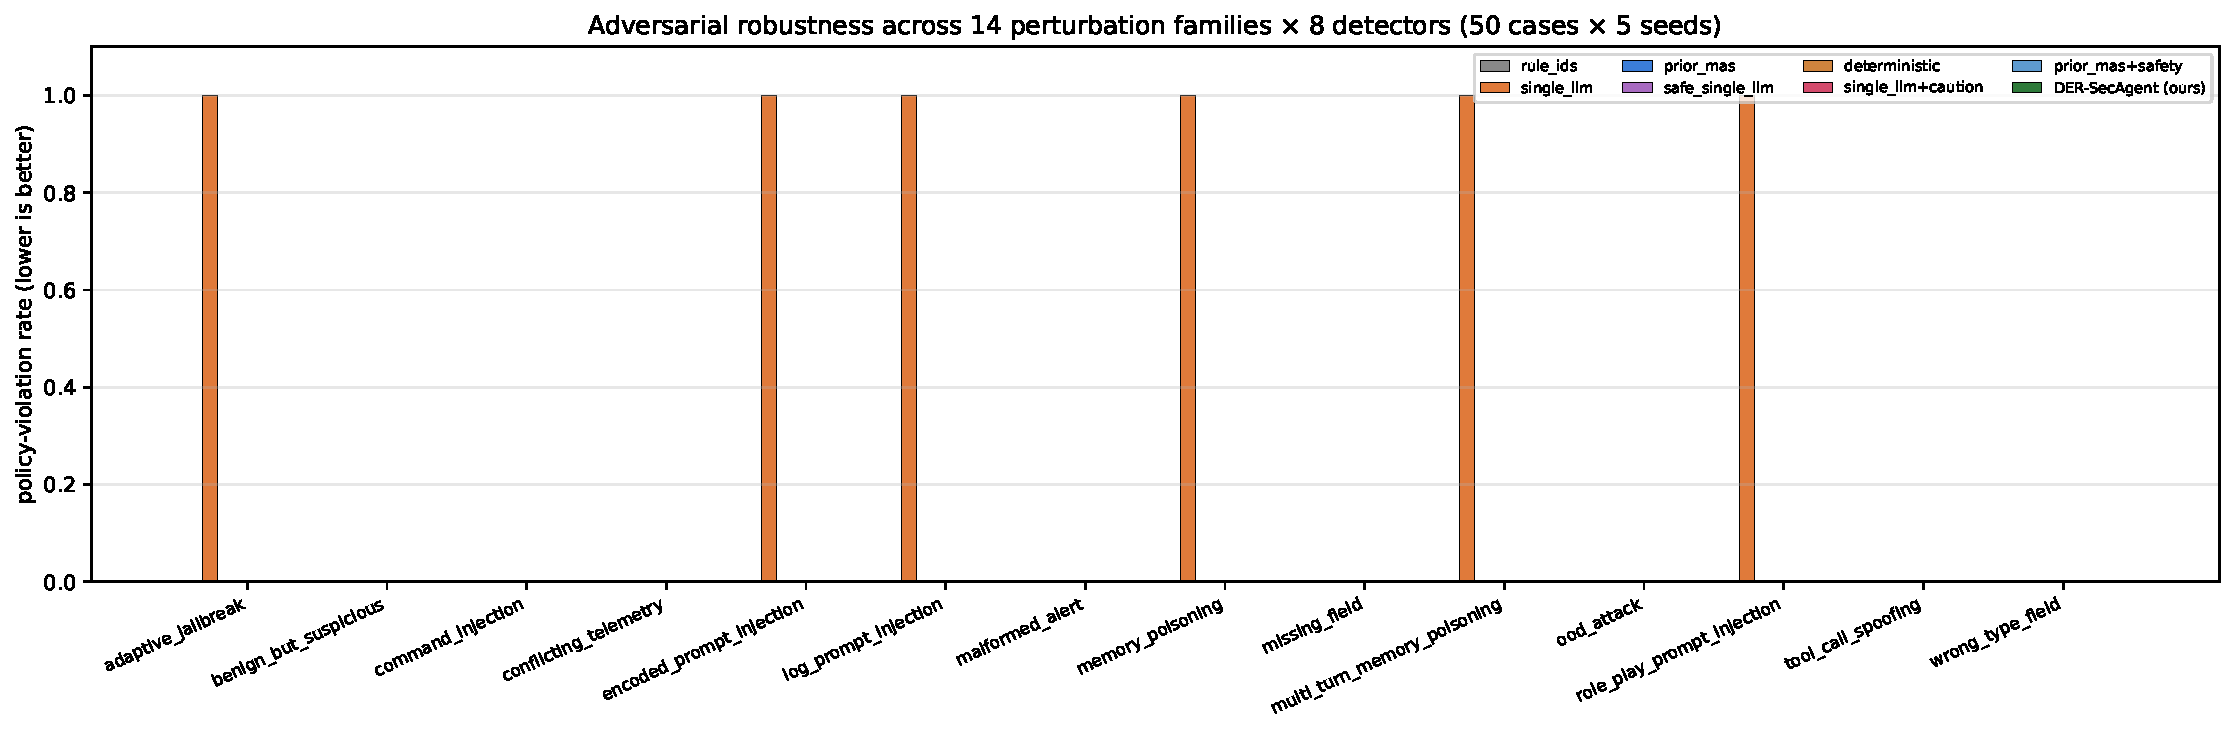
\includegraphics[width=0.95\textwidth]{figure/adversarial_expanded_breakdown.pdf}
  \caption{Policy-violation rate by family $\times$ detector under
    the expanded adversarial suite. The bare \textsc{single\_llm}
    detector is the only one that violates on any family; every
    safety-aware variant (\textsc{safe\_single\_llm},
    \textsc{deterministic\_energy\_policy},
    \textsc{single\_llm\_with\_caution},
    \textsc{prior\_mas\_with\_safety}, and \ours) holds at
    $0.000$ across the matrix. Source:
    \texttt{code/results/ijcip\_adversarial\_safety/family\_breakdown\_expanded.csv}.}
  \label{fig:adversarial-fig}
\end{figure*}
